\chapter{Introduction}
\label{cha:introduction}

\begin{comment}
All chapters should begin with an introduction before any sections, giving an overview of the chapter content.
Each section should in addition start with an introduction before its subsections begin.
Chapters with just one section --- or sections with just one sub-section --- should be avoided.
Think carefully about chapter and section titles as each title stands alone in the table of contents (without associated text)
and should convey the meaning of the contents of the chapter or section.

In all chapters and sections it is important to write clearly and concisely. Avoid repetitions and if needed refer back to the original discussion or presentation.
Each new section, subsection or paragraph should provide the reader with new information and be written in your own words. Avoid direct quotes.
If you use direct quotes, unless the quote itself is very significant, you are conveying to the reader that you are unable to express this discussion or fact yourself.
Such direct quotes also break the flow of the language (yours to someone else's).
\end{comment}

\section{Background and Motivation}\label{sec:background-and-motivation}
\label{sec:BackgroundAndMotivation}

\begin{comment}
Having a template to work from provides a starting point.
However, for a given project, a slight variation in the template may be required due to the nature of the given project.
Furthermore, the order in which the various chapters and sections will be written will also vary from project to project,
but the writing will seldom start at the abstract and sequentially follow the chapters of the report.
One critical reason for this is that you need to start writing as early as possible and that you will begin to write up where you are currently focusing.
However, do not leave working on the abstract until the very last days. The abstract is the first thing anyone reads of an article or thesis --- after the title;
and thus it is important that it is very well written. Abstracts are hard to write, so create revisions throughout the course of your project.

The background and motivation here should state where your project is situated in the field and what the key driving forces motivating this research are.
However, keep this section brief, as it is still part of the introduction.
The motivation will be further elaborated on in Chapter~\ref{cha:related_work}, presenting your complete state-of-the-art.

Note that this template uses italics to highlight where Latin wording is inserted to represent text and the text of the template
that we wish to draw your attention to. The italics themselves are not an indication that such sections should use italics.
\end{comment}

The field of \glspl{acr:llm} is an emerging one. \cite[2]{fanLargeLanguageModels2023} found that the proportion of papers about \glspl{acr:llm}\footnote{Including articles whose title or abstract includes \enquote{\acrshort{acr:llm}}, \enquote{\acrlong{acr:llm}}, or \enquote{\acrshort{acr:gpt}}.} to arXiv has skyrocketed since 2020, with a six-times increase in percent points from 2022 to 2023. Furthermore, they write that prompt engineering has been extensively used as a way to improve code generation \citep[7]{fanLargeLanguageModels2023}. \gls{acr:llm} technologies provide great opportunities for automation of tasks in a variety of fields, possibly also in the field of \gls{acr:gis} Data Analysis. With the capabilities of ChatGPT's Code Interpreter to generate, execute, and review its own code, research should be done to see if these capabilities can be applied to \gls{acr:gis}-related tasks.

\section{Goals and Research Questions}\label{sec:goals-and-research-questions}
\label{sec:GoalsandResearchQuestions}

\begin{comment}
A research project needs to have one or several question(s) that should be answered.
It is desirable to formulate such questions as early as possible as they provide both an important driving force for the project and clarity as to the goals sought.
However, expect to refine the questions and thus the final path of the project as work progresses.
Any refinements should be conducted with care, so as to avoid that the original aims and previous work are lost.
It is always good to have one (or max two) research goals and perhaps some subgoals,
together with 2--3 explicit research questions (or max four).

\begin{description}
    \item[Goal] \textit{Lorem ipsum dolor sit amet, consectetur adipiscing elit.}
\end{description}

Your goal/objective should be described in a single sentence.
In the text underneath it you can expand on this sentence to clarify what is meant by the short goal description.
The goal of your work is what you are trying to achieve. This can either be the goal of your actual project or
can be a broader goal that you have taken steps towards achieving. Such steps should be expressed in the research questions.
Note that the goal is seldom to build a system. A system is built to enable experiments to be conducted.
The research goal stages the needs that the system is implemented to meet.

\begin{description}
    \item[Research question 1] \textit{Lorem ipsum dolor sit amet, consectetur adipiscing elit.}
\end{description}

Each research question provides a sub-goal and these should be precise and clearly stated enabling the reader to match your results to the original goals.
They will also form the driving force for the experimental plan.

\begin{description}
    \item[Research question 2] \textit{Lorem ipsum dolor sit amet, consectetur adipiscing elit.}
\end{description}

Potentially, how well the goals have been met (and how well the research questions have been answered)
is a theme that you should return to towards the end of the thesis (so in Chapter~\ref{cha:conclusion} and/or Chapter~\ref{cha:discussion}).

For a Specialisation Project, the goal would primarily be to get up to speed with the research field, so the research questions will rather be
limited to exploring what the state-of-the-art is, what methods and data have been used, etc.
A secondary goal of the specialisation is to frame the research questions and goals of the Master's Thesis.
Note that a major difference between the Specialisation Project and the Master's Thesis is that the Master's Thesis work \textit{has\/} to
introduce new research.
Of course the Specialisation Project can also introduce novel work, but there is no such requirement --- and most commonly it does not,
since the core of the project really is to figure out what is ``old'' before you can introduce something which is new.
\end{comment}

The overarching goal of this specialization project is to investigate how \acrlongpl{acr:llm} can be utilized to make \gls{acr:gis} analysis simpler, faster, and more accessible. As exemplified in the task description provided by Norkart (see \cref{app:task-description}), such a system should be able to create a meaningful response to user queries such as:

\begin{quote}
    "Find all buildings within a 100-meter belt that are more than 100 meters above sea level and have docks."
\end{quote}

\noindent The task is then to investigate how \acrlongpl{acr:llm} can be utilized to perform classical \acrshort{acr:gis} analyses using standard \acrshort{acr:gis} technologies like PostGIS and geospatial data catalogues adhering to \acrshort{acr:ogc} or \acrshort{acr:stac} standards, in order to answer such a query.

Based on the task description, three research questions (RQs) have been constructed that this specialization project report will attempt to answer:

\begin{enumerate}
    \item What is the potential of \acrshort{acr:llm}-based \acrshort{acr:gis} analysis? \label{rq:llm-potential}
    \item How can \acrshort{acr:ogc} \acrshort{acr:api} - Features be used in an overlay analysis with ChatGPT-4? \label{rq:overlay-analysis}
    \item How can we give ChatGPT-4 access to external tools? \label{rq:external-tools}
\end{enumerate}

\rqref{rq:llm-potential} aims to assess the capabilities and limitations of integrating \glspl{acr:llm} with \glspl{acr:gis}. Researching the potential of using \glspl{acr:llm} in \gls{acr:gis} could uncover new methodologies for spatial analysis, predictive modelling, and decision-making.

\rqref{rq:overlay-analysis} focuses on the feasibility of using the \acrshort{acr:ogc} \acrshort{acr:api} - Features standard in a typical overlay analysis within a conversational \acrshort{acr:ai} context like ChatGPT-4, enabling users to express themselves using natural language queries. Examples of such analyses could be intersecting of map layers or filtering features based on certain criteria.

\rqref{rq:external-tools} delves into the technical considerations of expanding ChatGPT-4's capabilities through integration with external tools, such as \acrshort{acr:gis} software or data analytics platforms. It would also evaluate options for efficient data exchange, such as web \acrshortpl{acr:api}.

\begin{comment}

\section{Research Method}\label{sec:research-method}

% What methodology will you apply to address the goals: theoretic/analytic, model/abstraction or design/experiment?
% This section will describe the research methodology applied and the reason for this choice of research methodology.
% You should return to the actual choices made in the work and the alternatives in the Discussion chapter.

My research methods consist of a literature study and a set of experiments/proofs of concept, the latter of which is described in detail in \autoref{cha:experiments}.

\subsection{Literature Study}\label{subsec:research-method-literature-study}

I set out by deciding on some search terms, and used a "snowball sampling" technique to find relevant articles. \autoref{tbl:literature-search-results} shows the number of search results on various sites.

In order to evaluate large amounts of literature, a strategy of filtering out papers that are \textit{not} relevant was put in place. The strategy involves reading the least time-consuming and more information- packed sections first, and then reading other parts of the paper if it is deemed relevant to the project. \autoref{fig:searching-strategy} shows the order in which the different types of elements/sections commonly were read, and at any point in this pipeline the paper could be deemed irrelevant, and would subsequently be discarded from the literature study. The literature study is presented in \autoref{cha:related-work}.

\subsection{Experiments}\label{subsec:research-method-experiments}

Three experiments were conducted in order to answer the research questions listed in \autoref{sec:goals-and-research-questions}. As the literature study is the main focus of this specialization project, the experiments are not very in depth, but serve to support some of the claims that are made about the potential of an \acrshort{acr:llm}-based \acrshort{acr:gis} agent. The experiments is are presented in \autoref{cha:experiments}.

\begin{figure}
    \centering
    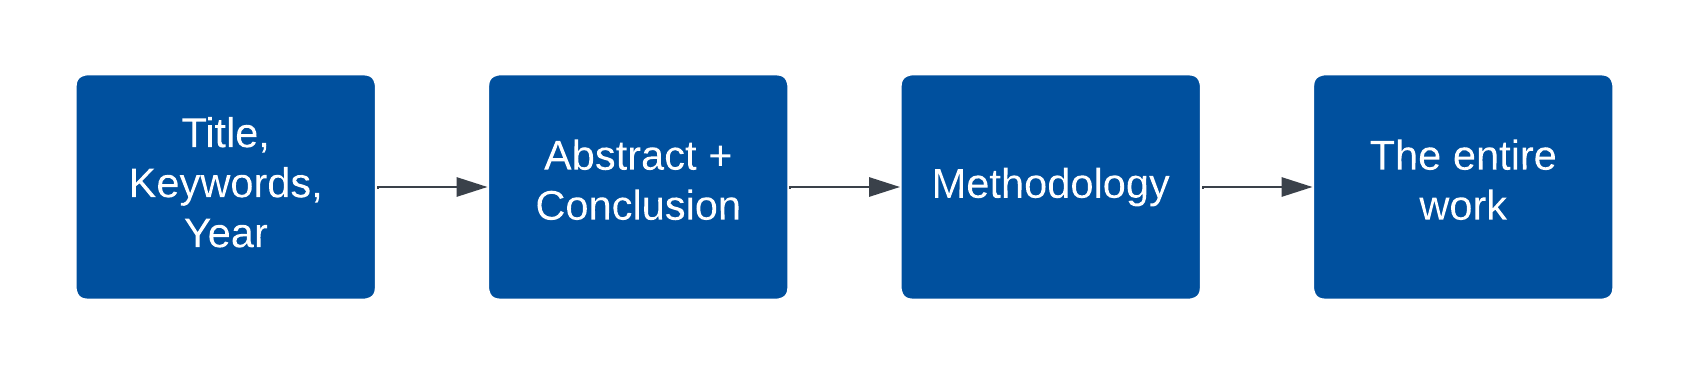
\includegraphics[width=\textwidth]{../figs/Literature study.png}
    \caption{Seaching strategy}
    \label{fig:searching-strategy}
\end{figure}



% \begin{table}
%     \centering
%     \begin{tabular}{p{5.5cm}|p{2cm}|p{2cm}|p{2cm}}
%         \toprule
%         Keyword  & arXiv  & Google Scholar & Web of Science \\
%         \midrule
%         \DTLforeach{literature_study}{
%             \Keyword=Keyword, \arXiv=arXiv, \GoogleScholar=GoogleScholar, \WebOfScience=WebOfScience}{
%         \Keyword & \arXiv & \GoogleScholar & \WebOfScience
%             \DTLiflastrow{}{\\}
%         }
%         \\
%         \bottomrule
%     \end{tabular}
%     \caption{Literature study search results}
%     \label{tbl:literature-search-results}
% \end{table}

\begin{table}
    \centering
    \begin{tabular}{p{5.5cm}|p{2cm}p{2cm}p{2cm}}
        \toprule
        \textbf{Keyword}               & \textbf{arXiv} & \textbf{Google Scholar} & \textbf{Web of Science} \\
        \midrule
        Large Language Model           & 5,101          & 5.76e6                  & 36,463                  \\
        Geographic Information System  & 588            & 7.36e6                  & 50,688                  \\
        Geospatial standard            & 55             & 295,000                 & 3,363                   \\
        Prompt engineering             & 1,081          & 1.02e6                  & 24,281                  \\
        Retrieval-augmented generation & 491            & 3,050                   & 19                      \\
        Text embedding                 & 4,730          & 402,000                 & 16,193                  \\
        LLM fine-tuning                & 917            & 10,200                  & 22                      \\
        \bottomrule
    \end{tabular}
    \caption{Literature study search results}
    \label{tbl:literature-search-results}
\end{table}
\end{comment}

\section{Contributions}
\label{sec:introContributions}

\begin{comment}
This section just provides a brief summary of the main contributions of the work.
The main description of the contributions will come in Section~\ref{sec:contributions}, after the results are presented.
(Hence Section~\ref{sec:introContributions} can also be left out, leaving the discussion completely to Section~\ref{sec:contributions}.)

The format of this section will generally be as follows:

\begin{enumerate}
    \item \textit{Lorem ipsum dolor sit amet, consectetur adipiscing elit.}
    \item \textit{Lorem ipsum dolor sit amet, consectetur adipiscing elit.}
    \item \textit{Lorem ipsum dolor sit amet, consectetur adipiscing elit.}
\end{enumerate}

\noindent
where the items on the list briefly describe the key contributions.

The order of the contributions here is important. List your main contribution first!
Creating this list will help you not only with writing the Conclusion (where all items listed here definitely should be included, and in more detail),
but also with items that need to be mentioned in the Abstract, as well as with points that you will want to bring to attention in the Discussion.
Hence most of the content on this list will be addressed 4--5 times in your text: here, in the Abstract, Discussion, Conclusion, and (most likely)
in the Results chapter.
\end{comment}

The main contributions of this specialization project are listed below:
\begin{enumerate}
    \item Gather relevant literature to facilitate development of state-of-the-art \acrshort{acr:llm}-based \acrshort{acr:gis} agents.
    \item Conduct tests on ChatGPT-4 to explore its proficiency in manipulating geospatial data across different formats and access channels.
\end{enumerate}

\section{Thesis Structure}
\label{sec:thesisStructure}

\begin{comment}
This section provides the reader with an overview of what is coming in the next chapters.
You want to say more than what is explicit in the chapter name, if possible, but still keep the description short and to the point. So something along the lines of:

\begin{itemize}
    \item Chapter~\ref{cha:background_theory} introduces the theory, tools and methods necessary to understand the work.
    \item \textit{Lorem ipsum dolor sit amet, consectetur adipiscing elit.}
    \item Chapter~\ref{cha:conclusion} sums up the work and points to ways it can be improved or extended in the future.
\end{itemize}
\end{comment}

The thesis is divided into four main sections:
\begin{itemize}
    \item \Autochapterref{cha:theory} lays the theoretical groundwork needed to understand the work.
    \item \Autochapterref{cha:related-work} discusses previous work related to the thesis.
    \item \Autochapterref{cha:experiments} explains the planning and setup for testing, and presents the results of the tests.
    \item \Autochapterref{cha:discussion-and-conclusion} discusses finding from the tests, suggests areas of importance when developing \acrshort{acr:llm}-based \acrshort{acr:gis} agents, and concludes the project report.
\end{itemize}

\glsresetall